\documentclass[11pt]{article}
\usepackage{latexsym}
\usepackage{amsmath,amssymb,amsthm}
\usepackage{epsfig}
\usepackage[right=0.8in, top=1in, bottom=1.2in, left=0.8in]{geometry}
\usepackage{setspace}

\usepackage{url}
\usepackage{natbib}
\usepackage[utf8]{inputenc}

\spacing{1.06}

\newcommand{\handout}[5]{
  \noindent
  \begin{center}
  \framebox{
    \vbox{\vspace{0.25cm}
      \hbox to 5.78in { {SE3352:\hspace{0.12cm}Algorithm Design} \hfill #2 }
      \vspace{0.48cm}
      \hbox to 5.78in { {\Large \hfill #5  \hfill} }
      \vspace{0.42cm}
      \hbox to 5.78in { {#3 \hfill #4} }\vspace{0.25cm}
    }
  }
  \end{center}
  \vspace*{4mm}
}
\newcommand{\lecture}[4]{\handout{#1}{#2}{#3}{Scribes:\hspace{0.08cm}#4}{Notes #1}}

\newtheorem{theorem}{Theorem}
\newtheorem{corollary}[theorem]{Corollary}
\newtheorem{lemma}[theorem]{Lemma}
\newtheorem{observation}[theorem]{Observation}
\newtheorem{example}[theorem]{Example}
\newtheorem{definition}[theorem]{Definition}
\newtheorem{claim}[theorem]{Claim}
\newtheorem{fact}[theorem]{Fact}
\newtheorem{assumption}[theorem]{Assumption}
\newcommand{\E}{\textbf{E}}
\newcommand{\var}{\text{var}}
\def\eps{\ensuremath\epsilon}
\begin{document}

\lecture{- Symmetric Encryption}{Dec 18, 2021}{Instructor:\hspace{0.08cm}\emph{Guoqiang Li}}{\emph{Qilong Lin, Huidong Xu}}


\section{Introduction}

This notes is organized as follows: In section 1 presents basic background of symmetric algorithms. Many concepts are defined academically in section 2. In section 3 provides three specific symmetric algorithms, namely DES, 3DES and AES. Industrial improvement based on AES algorithm is discussed in section 4. Key properties including algorithm complexity analysis presents in section 5. Finally, provide a conclusion in section 6.

\subsection{Background}

Nowadays, with the popularization of the Internet, more and more data is transmitted insecurely on the Internet, which just like a person running naked on the street. Encryption, which is defined as the process of encoding information in cryptography, can solve network transmission insecurity issues.

To be more specific, encryption\citep{Encryption} means converting the original representation of the information, known as \textbf{plaintext}, into an alternative form known as \textbf{ciphertext}. Ideally, only authorized parties can decipher a ciphertext back to plaintext and access the original information.

Symmetric encryption\citep{Symmetric_Encryption} is a type of encryption where only one key is used to both encrypt and decrypt electronic information. By using symmetric encryption algorithms, data is converted to a form that cannot be understood by anyone who does not possess the secret key to decrypt it, which ensures the security of data.	

\subsection{Application}
While symmetric encryption is an old method of encryption, it is \textbf{faster} and \textbf{more efficient} than asymmetric encryption, which takes a toll on networks due to performance issues with data size and heavy CPU use.

Due to the better performance and faster speed of symmetric encryption (compared to asymmetric), symmetric cryptography is typically used for bulk encryption and encrypting large amounts of data, e.g. for database encryption.

Some examples\citep{Symmetric_Encryption} of where symmetric cryptography is used are:

\begin{itemize}
    \item Payment applications, such as card transactions where PII needs to be protected to prevent identity theft or fraudulent charges.
    \item Validations to confirm that the sender of a message is who he claims to be.
    \item Random number generation or hashing.
    \item Encrypting data stored on a device when that data is not being transferred.
\end{itemize}

\subsection{Pros and Cons}

Compared to asymmetric cryption, symmetric cryption is faster to run because the keys used are much shorter than they are in asymmetric cryption. What's more, the fact that only one key gets used also makes the entire process faster.

However, symmetric also suffers from behavior where every use of a key \textit{leaks} some information that can potentially be used by an attacker to reconstruct the key, which may eventually causes the key to be cracked.

\section{Problem Description}
When we transfer our data through network, the sender will use \textbf{key} to encode the original data while the receiver will also use \textbf{key} to decode the encoded data.

\begin{definition}
[Key (cryptography)]
A piece of information, usually a string of numbers or letters that are stores in a file, which, when processed through a cryptographic algorithm, can encode or decode cryptographic data.
\end{definition}

\begin{definition}
[Symmetric-key algorithms]
Algorithms for cryptography that use the same cryptographic keys for both the encryption of plaintext and the decryption of ciphertext.
\end{definition}

Symmetric-key encryption can use either \textbf{stream ciphers} or \textbf{block ciphers}.

\begin{definition}
[Stream ciphers]
A type of symmetric-key algorithms which encrypt the digits (typically bytes), or letters (in substitution ciphers) of a message one at a time.
\end{definition}

\begin{definition}
[Block ciphers]
A type of symmetric-key algorithms which take a number of bits and encrypt them as a single unit, padding the plaintext so that it is a multiple of the block size.
\end{definition}

\begin{definition}
[Encryption]
The process of encoding data to prevent it from intruders to read the original data easily. This stage has the ability to convert the original data (plaintext) into unreadable format known as ciphertext.
\end{definition}

\begin{definition}
[Decryption]
The process to convert ciphertext into plaintext without missing any words in the original text.
\end{definition}

There are many specific algorithms for each type mentioned above, like \textbf{ChaCha20} for stream ciphers and \textbf{AES} for block ciphers. In the next part, I'd like to focus on \textbf{DES}, \textbf{3DES} and \textbf{AES}.

\section{Algorithms/Models}

\subsection{Data Encryption Standard (DES)}
DES is the archetypal block cipher - an algorithm that takes a fixed-length string or plaintext bits and transforms it through a series of complicated operations into another ciphertext bitstring of the same length. In the case of DES, the block size is 64 bits. DES also uses a key to customize the transformation, so that decryption can supposedly only be performed by those who know the particular key used to encrypt. The key ostensibly consists of 64 bits, however, only 56 of these are actually used by the algorithm. 8 bits are used solely for checking parity, and are thereafter discarded. Hence the effective key length is 56 bits. Decryptionuses the same structure as encryption, but with the keys used in reverse order.

\subsubsection{Overall Structure}
The algorithm's overall structure\citep{de2007analysis} is shown in Figure \ref{fig:des_procedure}. There are 16 identical stages of processing, termed \textit{round}. There is also an initial and final permutation, termed \textit{IP} and \textit{FP}, which are inverses.

Before the main rounds, the block is divided into two 32-bit halves and processed alternately. This criss-crossing is known as the Feistel scheme. The Feistel structure ensures that decryption and encryption are very similar processes - the only difference is that subkeys are applied in the reverse order then decrypting. The rest of the algorithm is identical. This greatly simplifies implementation, particularly in hardware, as there is no need for separate encryption and decryption algorithms.

\begin{figure}[h!]
\centering
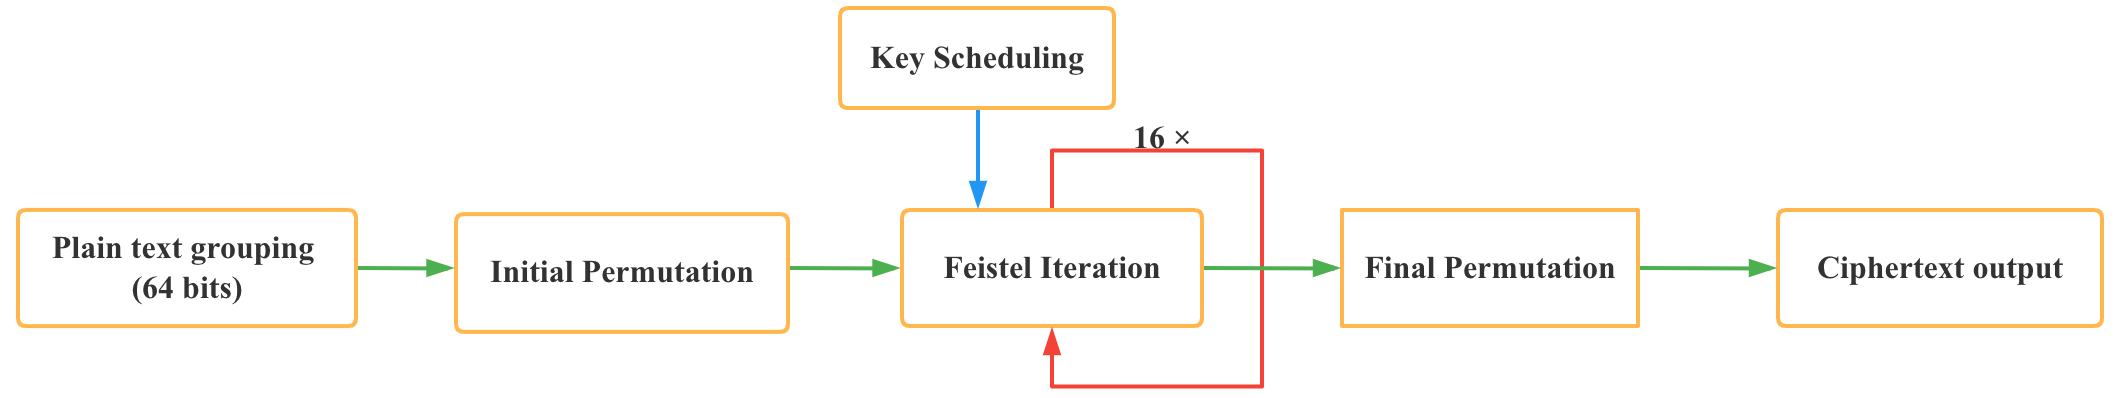
\includegraphics[scale=0.45]{des_procedure}
\caption{DES Procedure}
\label{fig:des_procedure}
\end{figure}

The algorithm's overall structure is shown in Figure below. There are 16 identical stages of processing, termed \textit{round}. There is also an initial and final permutation, termed \textit{IP} and \textit{FP}, which are inverses.

Before the main rounds, the block is divided into two 32-bit halves and processed alternately. This cross-crossing is known as the Feistel scheme. The Feistel structure ensures that decryption and encryption are very similar processes - the only difference is that subkeys are applied in the reverse order then decrypting. The rest of the algorithm is identical. This greatly simplifies implementation, particularly in hardware, as there is no need for separate encryption and decryption algorithms.

\subsubsection{Initial Permutation (IP)}

Initial Permutation disrupts the input bit sequence, that is, to exchange data at specific two positions. What's more, the inverse of the initial permutation is expressed as $IP^{-1}$, denoted as Final Permutation. IP and FP are public, have nothing to do with the key, and do not affect the security of DES.

\subsubsection{Feistel Function (F)}
The F-function operates on half a block (32 bits) at a time and consists of four stage.

\begin{enumerate}
    \item \textbf{\textit{Expansion}}: the 32-bit half-block is expanded to 48 bits using the expansion permutation, by duplicating half of the bits. The output consists of eight 6-bit (8 × 6 = 48 bits) pieces, each containing a copy of 4 corresponding input bits, plus a copy of the immediately adjacent bit from each of the input pieces to either side.
    \item \textbf{\textit{Key mixing}}: the result is combined with a subkey using an XOR operation. Sixteen 48-bit subkeys — one for each round — are derived from the main key using the key schedule (described below).
    \item \textbf{\textit{Substitution}}: after mixing in the subkey, the block is divided into eight 6-bit pieces before processing by the S-boxes, or substitution boxes. Each of the eight S-boxes replaces its six input bits with four output bits according to a non-linear transformation, provided in the form of a lookup table. The S-boxes provide the core of the security of DES — without them, the cipher would be linear, and trivially breakable.
    \item \textbf{\textit{Permutation}}: finally, the 32 outputs from the S-boxes are rearranged according to a fixed permutation, the P-box. This is designed so that, after permutation, the bits from the output of each S-box in this round are spread across four different S-boxes in the next round.
\end{enumerate}

\subsubsection{Key Schedule}

\begin{figure}[h!]
\centering
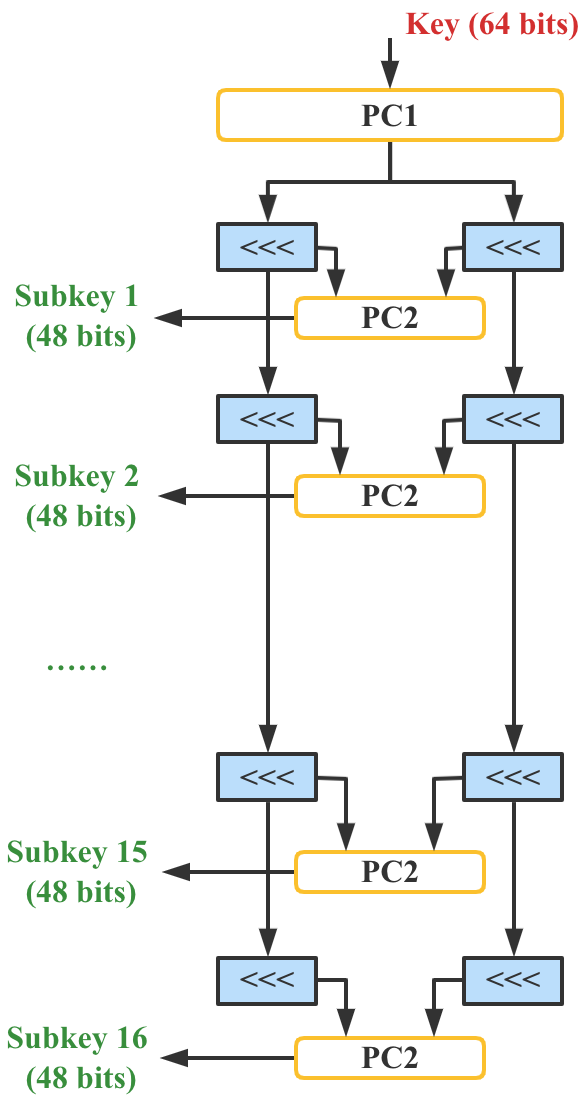
\includegraphics[width=0.45\textwidth,height=0.7\textwidth]{key_schedule}
\caption{Key Procedure}
\label{fig:key_schedule}
\end{figure}

Figure \ref{fig:key_schedule} illustrates the \textit{key schedule} for encryption - the algorithm which generates the subkeys.

Initially, 56 bits of the key are selected from the initial 64 by Permuted Choice 1 (PC-1) — the remaining eight bits are either discarded or used as parity check bits. The 56 bits are then divided into two 28-bit halves; each half is thereafter treated separately.

$$
\begin{aligned}
L_i &= R_{i - 1} \\ 
R_i &= L_{i - 1} + f(R_{i - 1}, K_{i}) \\
\end{aligned}
$$

In successive rounds, both halves are rotated left by one or two bits (specified for each round), and then 48 subkey bits are selected by Permuted Choice 2 (PC-2) — 24 bits from the left half, and 24 from the right. The rotations (denoted by "<<<" in the diagram) mean that a different set of bits is used in each subkey; each bit is used in approximately 14 out of the 16 subkeys.

The key schedule for decryption is similar—the subkeys are in reverse order compared to encryption. Apart from that change, the process is the same as for encryption. The same 28 bits are passed to all rotation boxes.

\subsection{Triple Data Encryption Standard (3DES)}

A symmetric-key block copher, which applies the DES cipher algorithm three times to each data block. The data Encryption Standard's (DES) 56-bit key is no longer considered adequate in the face of modern cryptanalytic techniques and supercomputing power.
	
3DES uses a \textbf{\textit{key bundle}} that comprises three DES keys, \textit{K1}, \textit{K2} and \textit{K3}, each of 56 bits (excluding parity bits). The encryption algorithm is:	

$$
ciphertext = E_{K3}(D_{K2}(E_{K1}(plaintext))).
$$

That is, DES encrypt with \textit{K1}, DES decrypt with \textit{K2}, then DES encrypt with \textit{K3}.
	
Decryption is the reverse:
$$
plaintext = D_{K1}(E_{K2}(D_{K3}(ciphertext))).
$$

That is, decrypt with \textit{K3}, encrypt with \textit{K2}, then decrypt with \textit{K3}.
	
Each triple encryption encrypts one block of 64 bits data.

In each case the middle operation is the reverse of the first and last. This improve the strength of the algorithm wehn using keying option 2 and provides backward compatibility with DES with keying option 3.

\subsection{Advanced Encryption Standard (AES)}

AES\citep{AES} is an iterative instead of Feistel cipher. It is based on two common techniques to encrypt and decrypt data knowned as substitution and permutation network (SPN). SPN is a number of mathematical operations that are carried out in block cipher algorithms.

AES has the ability to deal with 128 bits (16 bytes) as a fixed plaintext block size. These 16 bytes are represented in $4\times4$ matrix and AES operates on a matric of bytes:

$$
\left[
\begin{matrix}
b_0 & b_4 & b_8 & b_{12} \\
b_1 & b_5 & b_9 & b_{13} \\
b_2 & b_6 & b_10 & b_{14} \\
b_3 & b_7 & b_11 & b_{15} \\
\end{matrix}
\right]
$$

In addition, the number of rounds in AES is relied on the length of key:

\begin{itemize}
    \item 10 rounds for 128-bit keys.
    \item 12 rounds for 192-bit keys.
    \item 14 rounds for 256-bit keys.
\end{itemize}

The Figure \ref{fig:aes_procudure} below represents the basic structure of AES.

\begin{figure}[h!]
\centering
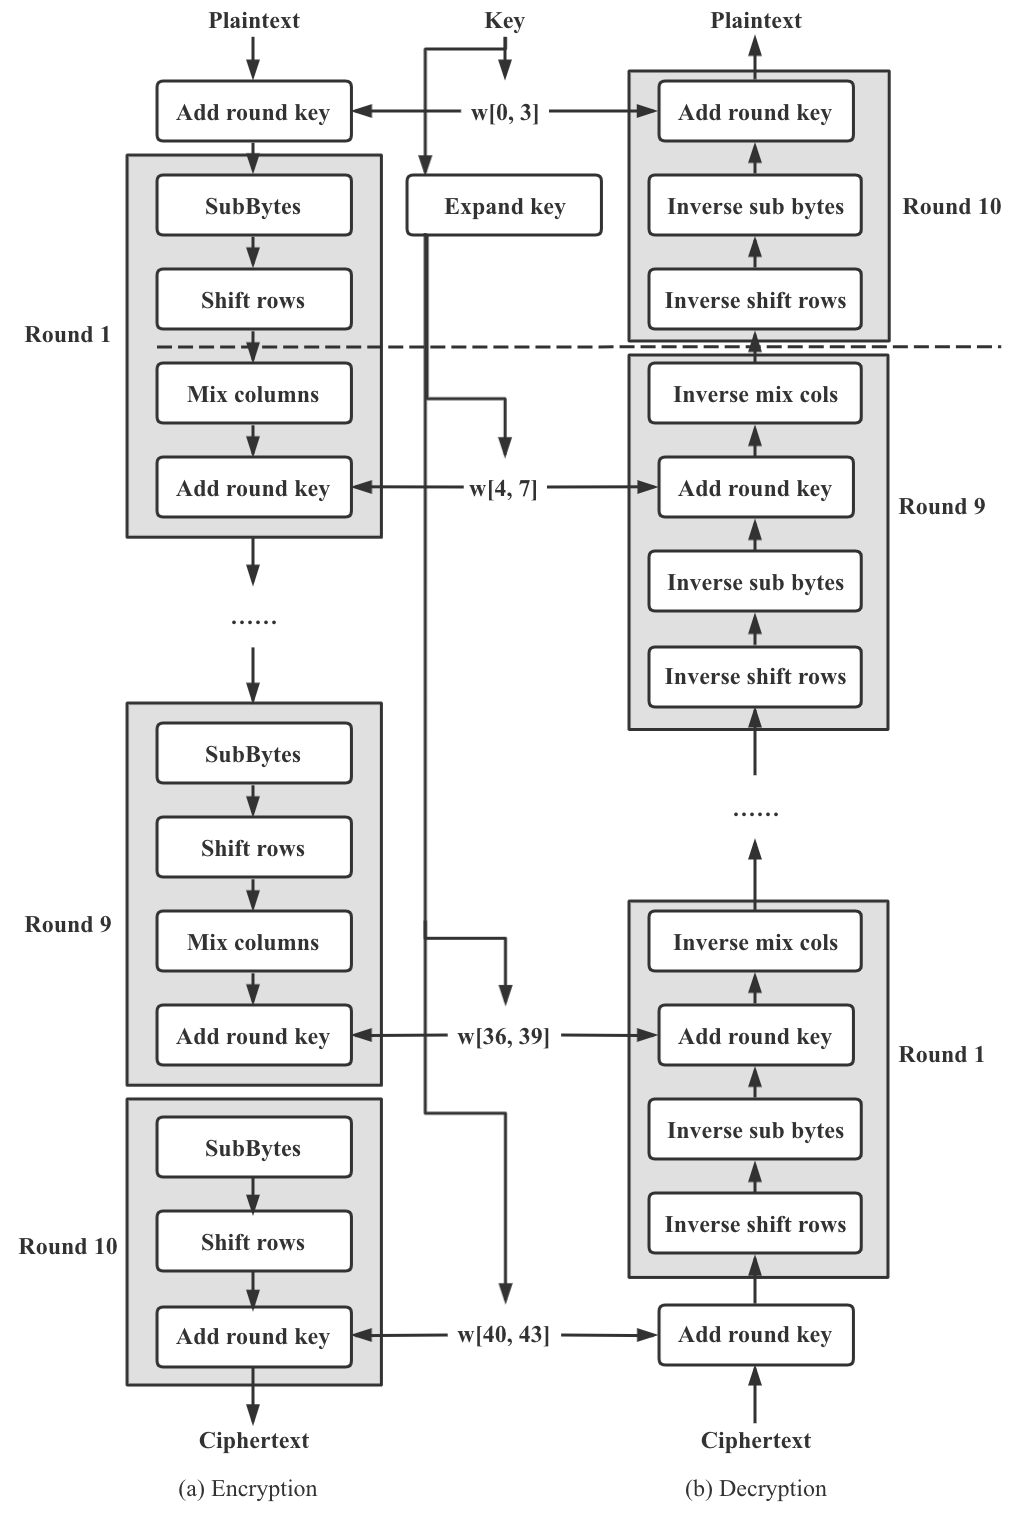
\includegraphics[scale=0.5]{aes_procudure}
\caption{AES Procedure}
\label{fig:aes_procudure}
\end{figure}

\subsubsection{The Substitute Bytes Step}

\begin{figure}[h!]
\centering
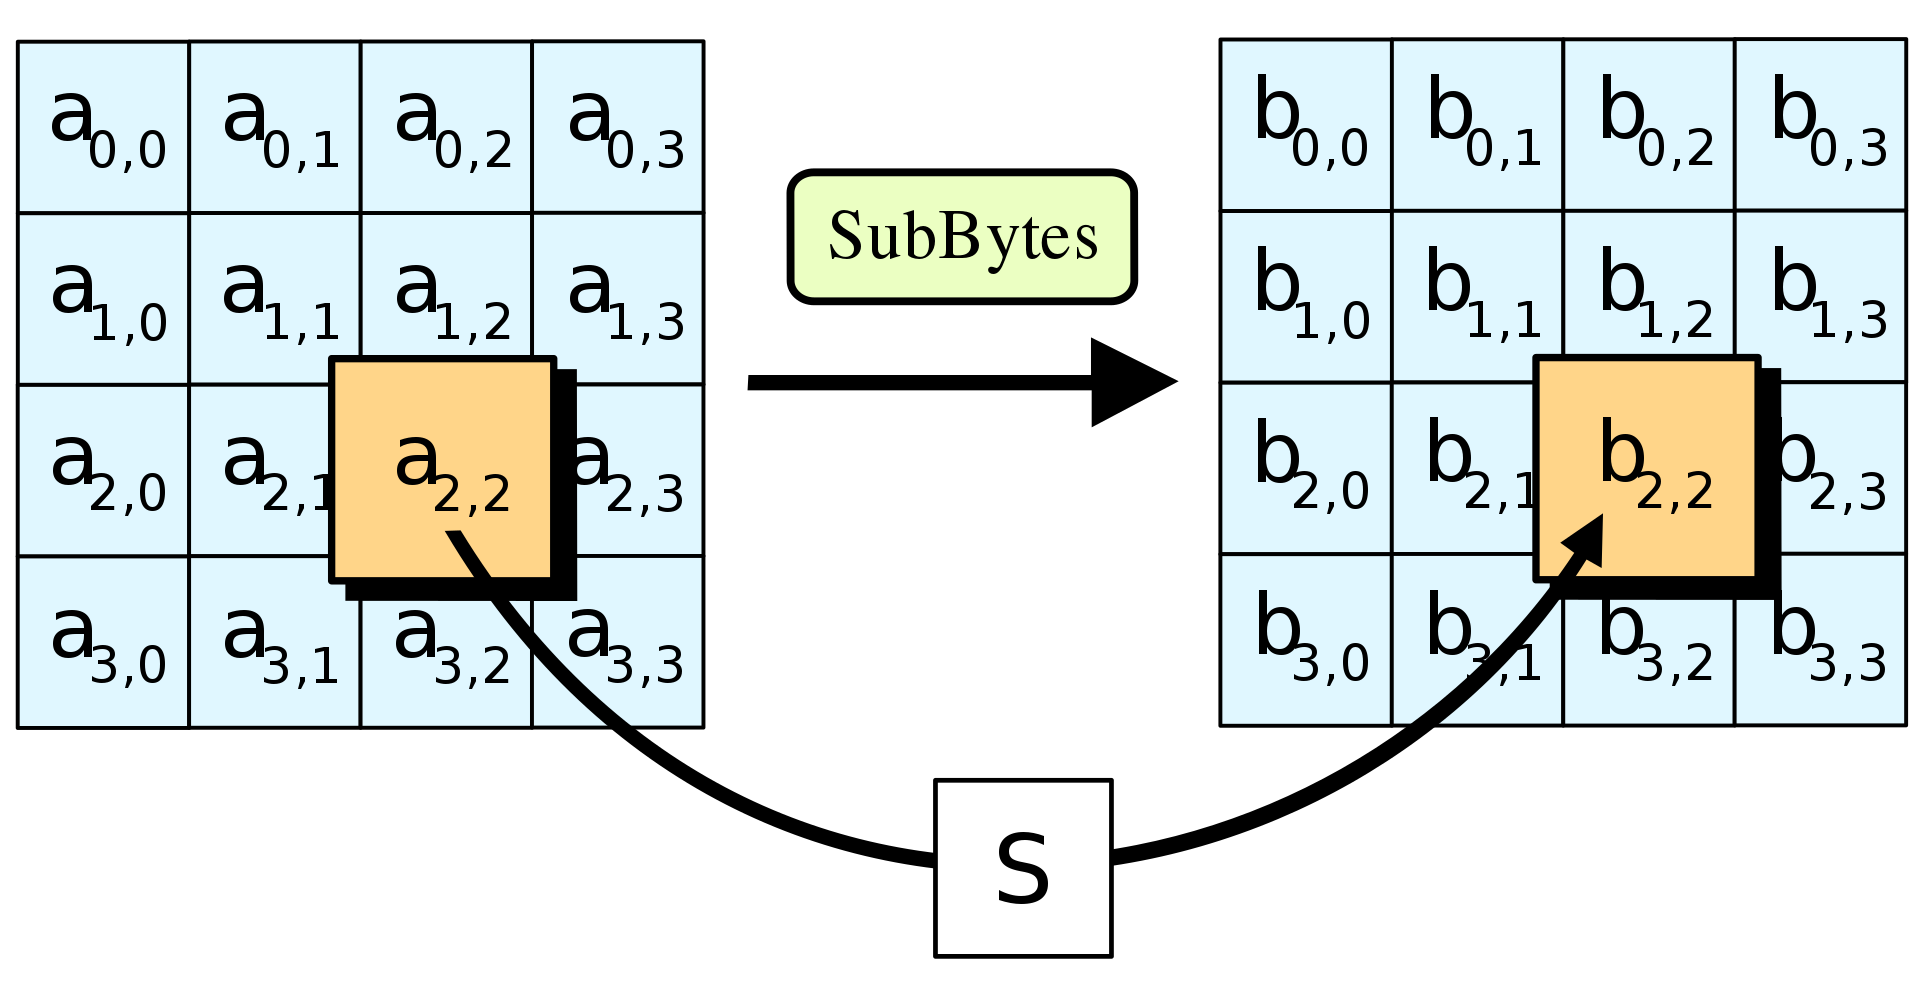
\includegraphics[scale=0.20]{subbytes}
\caption{SubBytes}
\label{fig:subbytes}
\end{figure}

In the SubBytes step, each byte $a_{i, j}$ in the state array is replaced with a SubBytes $S(a_{i, j})$ using an 8-bit substitution box. Note that before round 0, the \textit{state} array is simply the plaintext or input. This operation provides the non-linearity in the cipher. The S-box used is derived from the multiplicative inverse over GF($2^8$), known to have good non-linearity properties. To avoid attacks based on simple algebraic properties, the S-box is constructed by combining the inverse function with an invertible affine transformation. The S-box is also chosen to avoid any fixed points (and so is a derangement), i.e., $S(a_{i, j}) \neq a_{i, j}$, and also any opposite fixed points, i.e., $S(a_{i, j}) \bigoplus a_{i, j} \neq FF_{16}$. While performing the decryption, the InvSubBytes step (the inverse of SubBytes) is used, which requires first taking the inverse of the affine transformation and then finding the multiplicative inverse.

\subsubsection{The ShiftRows step}

The ShiftRows step operates on the rows of the state; it cyclically shifts the bytes in each row by a certain offset. For AES, the first row is left unchanged. Each byte of the second row is shifted one to the left. Similarly, the third and fourth rows are shifted by offsets of two and three respectively. In this way, each column of the output state of the ShiftRows step is composed of bytes from each column of the input state. The importance of this step is to avoid the columns being encrypted independently, in which case AES would degenerate into four independent block ciphers.

\subsubsection{The MixColumns step}

In the MixColumns step, the four bytes of each column of the state are combined using an invertible linear transformation. The MixColumns function takes four bytes as input and outputs four bytes, where each input byte affect all four output bytes. Together with ShiftRows, Mix Columns provides diffusion in the cipher.

During this operation, each column is transformed using a fixed matrix (matrix left-multiplied by column gives new value of column in the state):

$$
\begin{bmatrix}
b_{0, j} \\
b_{1, j} \\
b_{2, j} \\
b_{3, j}
\end{bmatrix}
=
\begin{bmatrix}
2 & 3 & 1 & 1 \\
1 & 2 & 3 & 1 \\
1 & 1 & 2 & 3 \\
3 & 1 & 1 & 2 
\end{bmatrix}
\quad
0 \leq j \leq 3
$$

Matrix multiplication is composed of multiplication and addition of the entries. Entries are bytes treated as coeffiecients of polynomial of order $x^7$. Addition is simply XOR. Multiplication is modulo irreducible polynomial $x^8 + x^4 + x^3 + x + 1$. If processed bit by bit, then, after shifting, a conditional XOR with $1B_{16}$ should be performed if the shifted value is larger than $FF_{16}$ (overflow must be corrected by substraction of generating polynomial). These are special cases of the usual multiplication in $GF(2^8)$.

In more general sense, each column is trated as a polynomial over $GF(2^8)$ and is then multiplied modulo $01_{16} \cdot z^4 + 01_{16}$ with a fixed polynomial $c(z) = 03_{16} \cdot z^3 + 01_{16} \cdot z^2 + 01_{16} \cdot z + 02_{16}$. The coefficients are displayed in their hexadecimal equivalent of the binary representation of bit polynomials from $GF(2)[x]$. The MixColumns step can also be viewed as a multiplication by the shown particular MDS matrix in the finite field $GF(2^8)$. This process is described further in the artical Rijndael MixColumns.

\subsubsection{The AddRoundKey step}

In the AddRoundKey step, the subkey is combined with the state. For each round, a subkey is derived from the main key using Rijndael's key schedule; each subkey is the same size as the state. The subkey is added by combining each byte of the state with the corresponding byte of the subkey using bitwise XOR.

\subsubsection{Optimization of the cipher}

On systems with 32-bit or larger words, it is possible to speed up execution of this cipher by combining the SubBytes and ShiftRows steps with the MixColumns step by transforming them into a sequence of table lookups. This requires four 256-entry 32-it tables (together occupying 4096 bytes). A round can then be performed with 16 table lookup operations and 12 32-bit exclusive-or operations, followed by four 32-bit exclusive-or operations in the AddRoundKey step. Alternatively, the table lookup operation can be performed with a single 256-entry 320bit table (occupying 1024 bytes) followed by circular rotation operations.

Using a byte-oriented approach, it is possible to combine the \textbf{SubBytes}, \textbf{ShiftRows}, and \textbf{MixColumns} steps into a single round operation.

\section{Practical Algorithm}
Symmetric encryption algorithms are used in many different fields in industry. The following mainly describes the application of symmetric encryption algorithm in the process of image encryption\citep{zeghid2007modified}.

\subsection{The performance index of gray image encryption algorithm}
For a gray scale image encryption algorithm, there are mainly these considerations in the industry:
\begin{itemize}
\item The \textbf{horizontal and vertical correlation} of the encrypted images
\item The \textbf{entropy} of the encrypted images
\item The \textbf{PSNR} of the encryption
\end{itemize}
Specifically, the above indicators are defined as follows:
\begin{definition}
A \textbf{gray scale image} is a $n \times m$ matrix $G$, and the values in the matrix is limited to range from 0 to 255. For convenience, we will still used this sign in the following definitions, and used $G(i, j)$ to represent the value at index $(i, j)$
\end{definition}
\begin{definition}
The \textbf{vertical correlation} of a gray scale image is the covariance of some randomly chosen vertical pixel pair.
\end{definition}
The process of obtaining the vertical correlation is as follows:
\begin{itemize}
\item Randomly select n pairs of two vertically adjacent pixels $a = G(i, j)$ and $b = G(i+1, j)$, put $a$ and $b$ into sets $A$ and $B$
\item Create two discrete random variable $X$ and $Y$, their value are randomly chosen from $A$ and $B$ respectively
\item Calculate the correlation coefficient of $X$ and $Y$
\end{itemize}
The correlation coefficient we get is the vertical correlation defined above.  The definition of \textbf{horizontal correlation} is almost the same, just randomly get horizontal adjacent pixels in the first step.

\begin{definition}
The \textbf{entropy} of a gray scale image G is written as:
\end{definition}

$$
H(G)=-\sum_{i=0}^{255}p(x_i)\log_2(p(x_i))
$$
Where $p(x_i)$ is the frequency of the value $i$ in the matrix $G$\\
Intuitively, the above 2 definitions correspond to the degree of visual confusion in the image, they can be used as an indicator of the difficulty of cracking.

\begin{definition}
The \textbf{Peak signal-to-noise ratio (PSNR)} of a gray scale image G is used to measure the quality of compression.
\end{definition}

Firstly, we need to define the \textbf{mean-square error (MSE)} of the origin image $I$ and the encrypted image $K$:
$$
MSE_{I,\ K}=\frac{1}{mn}\sum_{i=0}^{m-1}\sum_{j=0}^{n-1}[I(i,\ j)-K(i,\ j)]^2
$$
Then the peak signal-to-noise ratio can be defined as follows:
$$
PSNR_{I,\ K}=20\log_{10}(\frac{255}{\sqrt{MSE_{{I,\ K}}}})
$$
PSNR is most commonly used to measure the quality of reconstruction of lossy compression codecs. In our context, intuitively, the peak signal-to-noise ratio can be used to indicate the perception of the difficulty of restoring the encrypted image to the original image. The lower the PSNR, the more difficult it is to restore.

\subsection{Problems encountered in applying AES directly to gray scale image encryption}
In general, AES can be used to encrypt gray scale images directly, which can be seen from the following points:
\begin{itemize}
\item Statistic the gray value of each pixel of the encrypted image obtained by AES, and the frequency histogram of gray value can be obtained. Generally speaking, the frequency histogram of the encrypted image is quite different from that of the original image. And. In the frequency histogram of the encrypted image, the frequency of each gray value is basically the same, which makes it difficult for the attacker to find a breakthrough in this aspect.
\item Generally, the key space of AES encryption is very large, and even if two keys are used to encrypt the same image, the result of encryption will be very different, that is, sensitive to the Key. This ensures the security of the algorithm to a large extent.
\end{itemize}
However, for some special cases, simply using the AES encryption algorithm can be problematic. Consider using \textbf{Electronic Codebook Book (ECB)} mode for encryption, where the same data is encrypted to the same value. Therefore, if the image contains blocks of uniform color, these uniform blocks will be identical after encryption. Intuitively, \textbf{texture zones} will appear in the encrypted image. At this time, the entropy of the image is relatively low, and it is easier to crack.

\subsection{Use the improved AES algorithm to encrypt gray image}
To solve the problems mentioned above, we can combine the AES algorithm with \textbf{stream ciphers}. Stream cipher is an algorithm that continuously generates keys based on the internal state of the key and algorithm.\\
A simple understanding of why this is done solves the problem above: Originally, we used the key directly for each block of data. With the introduction of stream ciphers, instead of encrypting each block of data directly with the key, we use a series of keys generated by stream ciphers to encrypt the block of data. In this way, we can avoid texture zones on the image.

\subsection{The performance of improved AES algorithm to encrypt grayscale image}
As to which streaming ciphers to use in combination with AES, \textbf{A5/1 and W7} are mainly considered in the references (there is no explanation as to why these two algorithms were chosen, as they may have been found to perform better in practice). Table \ref{Tab34} indicates the performance of AES algorithm for encrypting grayscale images after combining the two algorithms:

\begin{table}[htbp]
\centering
\caption{Performance Comparison}
\label{Tab34}
\begin{tabular}{|l|l|l|l|}
\hline
Encryption algorithm   & AES   & AES+A5/1 & AES+W7  \\ \hline
Correlation vertical   & 0.066 & 0.077    & 0.03    \\ \hline
Correlation Horizontal & 0.046 & 0.056    & 0.02    \\ \hline
PSNR                   & 6.88  & 6.83     & 6.77    \\ \hline
Entropy                & 7.91  & 7.96     & $\sim$8 \\ \hline
\end{tabular}
\end{table}

It can be seen that the improved AES algorithm improves the information entropy of the encrypted image and reduces the PSNR. Among them, AES algorithm combined with W7 can reduce horizontal and vertical correlation very well.

\section{Key properties}

\subsection{Kerckhoofs' Principle}

Kerckhoffs' Principle\citep{Petitcolas2011} states that the security of a cryptosystem must lie in the choice of its keys only; everything else (including the algorithm itself should be considerded public knowledge.

The six principles enunciated by Kerckhoffs are as follows:

\begin{enumerate}
    \item The system must be substantially, if not mathematically, undecipherable.
    \item The system must not require secrecy and can be stolen by the enemy without causing trouble.
    \item It must be easy to communicate and remember the keys without requiring written notes, and it must also be easy to change or modify the keys with different participants.
    \item The system ought to be compatible with telegraph communication.
    \item The system must be portable, and its use must not require more than one person.
    \item Finally, regarding the circumstances in which such system is applied, it must be easy to use and must neither require stress of mind nor the knowledge of a long series of rules.
\end{enumerate}

\section{Conclusion}

\subsection{Future direction}
Symmetric encryption algorithms have been used in many fields, such as the image encryption field mentioned above. But what about the future direction?\\
Considering how to better improve the hardware resources required by symmetric encryption algorithm may be one of the important directions. Because in practical applications, besides the security of the algorithm, the speed of encryption and the hardware resources required by encryption are also important indicators.\\
Another possible future direction is cloud servers. In today's popular cloud servers, encryption is essential because many steps in cloud server rely on network transport. In the cloud service scenario (for example, users want their data to be hosted by the cloud server), how to design more efficient encryption algorithm is also an important direction.zhn

\subsection{Open problems}
There are still many problems in the application of symmetric encryption algorithm. In the specific implementation of symmetric encryption, the use of hardware resources is also an important indicator, which leads to many cases, we want to evaluate the quality of a symmetric encryption algorithm, may need to specific hardware to achieve it, in order to get the precise value of each indicator. In other words, our evaluation of algorithm results is more practice-dependent. How to explain theoretically why an algorithm is better can be a difficult task.

\bibliographystyle{plain}
\bibliography{references}

\end{document}
